\documentclass[11pt]{article}
\usepackage[margin=0.8in]{geometry}
\usepackage[T1]{fontenc}
\usepackage[utf8]{inputenc}
\usepackage{hyperref}
\usepackage{xcolor}
\usepackage{tikz}
\usetikzlibrary{arrows.meta,positioning,shapes.geometric,fit,backgrounds}
\usepackage{listings}
\usepackage{longtable}
\usepackage{booktabs}
\usepackage{enumitem}

\lstdefinestyle{code}{
  basicstyle=\ttfamily\scriptsize,
  breaklines=true,
  frame=single,
  columns=fullflexible,
  keepspaces=true,
  showstringspaces=false
}

\title{Llama 7B Forward Pass Compute Graph\\\large Color Dataflow View + Current File Structure}
\author{llama\_inference\_cpp}
\date{\today}

\begin{document}
\maketitle
\tableofcontents
\newpage

\section{What this graph shows}
This document visualizes the forward-pass compute graph in a color-coded way:
\begin{itemize}[leftmargin=*]
  \item each colored node is a function/kernel stage,
  \item arrows show tensor flow from one stage to the next,
  \item labels show main tensors produced and consumed,
  \item repeated per-layer block is explicitly indicated.
\end{itemize}

\section{Color legend}
\begin{itemize}[leftmargin=*]
  \item \textcolor{blue!70!black}{Blue}: input / embedding / output boundaries
  \item \textcolor{green!50!black}{Green}: normalization operations
  \item \textcolor{orange!80!black}{Orange}: linear projections (matvec)
  \item \textcolor{purple!70!black}{Purple}: positional encoding + attention internals
  \item \textcolor{red!70!black}{Red}: nonlinearity and sampling
\end{itemize}

\section{High-level compute graph (single token step)}
\begin{center}
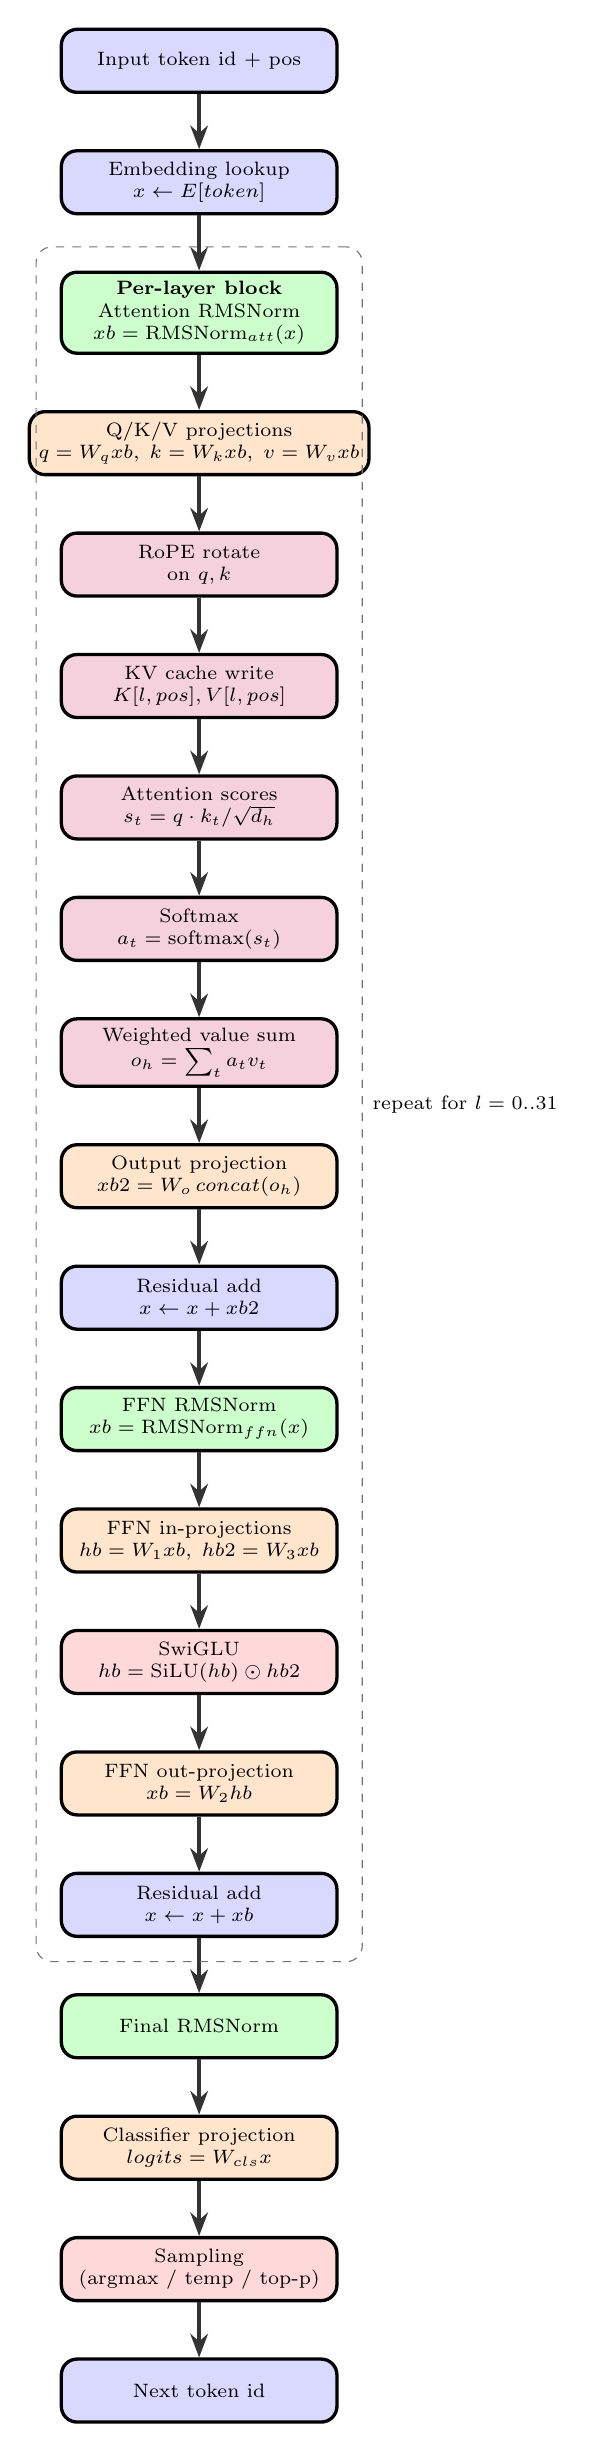
\begin{tikzpicture}[
  node distance=7mm and 6mm,
  >={Stealth[length=3mm]},
  every node/.style={font=\scriptsize, align=center},
  input/.style={draw, rounded corners=2mm, very thick, fill=blue!15, minimum width=35mm, minimum height=8mm},
  norm/.style={draw, rounded corners=2mm, very thick, fill=green!20, minimum width=35mm, minimum height=8mm},
  linear/.style={draw, rounded corners=2mm, very thick, fill=orange!20, minimum width=35mm, minimum height=8mm},
  attn/.style={draw, rounded corners=2mm, very thick, fill=purple!18, minimum width=35mm, minimum height=8mm},
  nonlin/.style={draw, rounded corners=2mm, very thick, fill=red!15, minimum width=35mm, minimum height=8mm},
  arrow/.style={->, very thick, color=black!80}
]

\node[input] (tok) {Input token id + pos};
\node[input, below=of tok] (embed) {Embedding lookup\\$x \leftarrow E[token]$};

\node[norm, below=of embed] (attn_norm) {\textbf{Per-layer block}\\Attention RMSNorm\\$xb = \mathrm{RMSNorm}_{att}(x)$};
\node[linear, below=of attn_norm] (qkv) {Q/K/V projections\\$q=W_qxb,\;k=W_kxb,\;v=W_vxb$};
\node[attn, below=of qkv] (rope) {RoPE rotate\\on $q,k$};
\node[attn, below=of rope] (kvwrite) {KV cache write\\$K[l,pos],V[l,pos]$};
\node[attn, below=of kvwrite] (scores) {Attention scores\\$s_t=q\cdot k_t/\sqrt{d_h}$};
\node[attn, below=of scores] (sm) {Softmax\\$a_t=\mathrm{softmax}(s_t)$};
\node[attn, below=of sm] (wsum) {Weighted value sum\\$o_h=\sum_t a_t v_t$};
\node[linear, below=of wsum] (wo) {Output projection\\$xb2=W_o\,concat(o_h)$};
\node[input, below=of wo] (res1) {Residual add\\$x \leftarrow x+xb2$};

\node[norm, below=of res1] (ffn_norm) {FFN RMSNorm\\$xb=\mathrm{RMSNorm}_{ffn}(x)$};
\node[linear, below=of ffn_norm] (w13) {FFN in-projections\\$hb=W_1xb,\;hb2=W_3xb$};
\node[nonlin, below=of w13] (swiglu) {SwiGLU\\$hb=\mathrm{SiLU}(hb)\odot hb2$};
\node[linear, below=of swiglu] (w2) {FFN out-projection\\$xb=W_2hb$};
\node[input, below=of w2] (res2) {Residual add\\$x\leftarrow x+xb$};

\node[norm, below=of res2] (finaln) {Final RMSNorm};
\node[linear, below=of finaln] (cls) {Classifier projection\\$logits=W_{cls}x$};
\node[nonlin, below=of cls] (sample) {Sampling\\(argmax / temp / top-p)};
\node[input, below=of sample] (next) {Next token id};

\draw[arrow] (tok) -- (embed);
\draw[arrow] (embed) -- (attn_norm);
\draw[arrow] (attn_norm) -- (qkv);
\draw[arrow] (qkv) -- (rope);
\draw[arrow] (rope) -- (kvwrite);
\draw[arrow] (kvwrite) -- (scores);
\draw[arrow] (scores) -- (sm);
\draw[arrow] (sm) -- (wsum);
\draw[arrow] (wsum) -- (wo);
\draw[arrow] (wo) -- (res1);
\draw[arrow] (res1) -- (ffn_norm);
\draw[arrow] (ffn_norm) -- (w13);
\draw[arrow] (w13) -- (swiglu);
\draw[arrow] (swiglu) -- (w2);
\draw[arrow] (w2) -- (res2);
\draw[arrow] (res2) -- (finaln);
\draw[arrow] (finaln) -- (cls);
\draw[arrow] (cls) -- (sample);
\draw[arrow] (sample) -- (next);

\node[draw=black!55, dashed, rounded corners=2mm, fit=(attn_norm)(res2), inner sep=3mm, label={[black]right:repeat for $l=0..31$}] {};

\end{tikzpicture}
\end{center}

\section{Kernel/function mapping table}
\begin{longtable}{p{0.24\linewidth} p{0.33\linewidth} p{0.36\linewidth}}
\toprule
\textbf{Stage} & \textbf{Implementation call} & \textbf{Primary output} \\
\midrule
\endhead
Embedding & CPU copy in engine & \texttt{x[dim]} \\
Attention norm & \texttt{launch\_rmsnorm} & \texttt{xb[dim]} \\
Q projection & \texttt{launch\_matvec(Wq)} & \texttt{q[dim]} \\
K projection & \texttt{launch\_matvec(Wk)} & \texttt{k[kv\_dim]} \\
V projection & \texttt{launch\_matvec(Wv)} & \texttt{v[kv\_dim]} \\
RoPE & \texttt{launch\_rope\_qk} & rotated \texttt{q,k} \\
Attention scores & \texttt{launch\_attention\_scores} & \texttt{scores[t]} \\
Softmax & \texttt{launch\_softmax\_inplace} & \texttt{att[t]} \\
Value mix & \texttt{launch\_attention\_weighted\_sum} & head output \\
Attention out proj & \texttt{launch\_matvec(Wo)} & \texttt{xb2[dim]} \\
FFN norm & \texttt{launch\_rmsnorm} & \texttt{xb[dim]} \\
FFN W1/W3 & \texttt{launch\_matvec(W1/W3)} & \texttt{hb, hb2} \\
SwiGLU & \texttt{launch\_swiglu} & gated \texttt{hb} \\
FFN W2 & \texttt{launch\_matvec(W2)} & \texttt{xb[dim]} \\
Final norm & \texttt{launch\_rmsnorm} & normalized \texttt{x} \\
Classifier & \texttt{launch\_matvec(Wcls)} & \texttt{logits[vocab]} \\
Sampling & CPU sampler & \texttt{next token id} \\
\bottomrule
\end{longtable}

\section{Current file structure used}
Snapshot source:
\texttt{docs/FILE\_STRUCTURE\_SNAPSHOT.txt}

\lstinputlisting[style=code]{FILE_STRUCTURE_SNAPSHOT.txt}

\section{Where each part lives}
\begin{itemize}[leftmargin=*]
  \item Engine core: \texttt{src/llama\_engine.cpp}
  \item CLI entrypoint: \texttt{src/main.cpp}
  \item CUDA kernel API: \texttt{include/cuda\_kernels/llama\_cuda\_kernels.cuh}
  \item CUDA kernels (modular): \texttt{src/cuda\_kernels/*.cu}
  \item Handbooks: \texttt{docs/}
\end{itemize}

\end{document}
